\documentclass[11pt, oneside]{article}   	% use "amsart" instead of "article" for AMSLaTeX format
\usepackage{geometry}                		% See geometry.pdf to learn the layout options. There are lots.
\geometry{letterpaper}                   		% ... or a4paper or a5paper or ... 
%\geometry{landscape}                		% Activate for for rotated page geometry
%\usepackage[parfill]{parskip}    		% Activate to begin paragraphs with an empty line rather than an indent
\usepackage{graphicx}				% Use pdf, png, jpg, or eps� with pdflatex; use eps in DVI mode
								% TeX will automatically convert eps --> pdf in pdflatex		
\usepackage{amssymb}
\usepackage{amsmath}
\usepackage{parskip}
\usepackage{color}

\title{Complex numbers for computation}
%\author{The Author}
%\section{}
% \subsection*{R code}
\date{}							% Activate to display a given date or no date

\graphicspath{{/Users/telliott_admin/Dropbox/Tex/png/}}

% \begin{center} 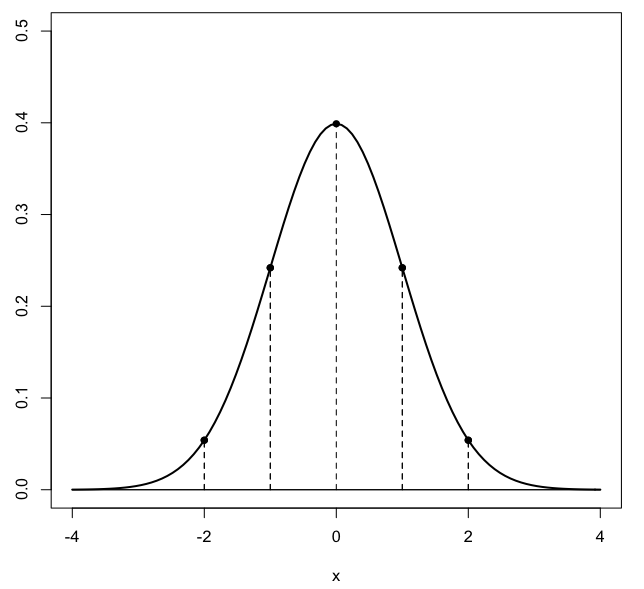
\includegraphics [scale=0.4] {gauss3.png} \end{center}

\begin{document}
\maketitle
\Large
Fitzpatrick's book on Mechanics (Chapter 7) uses complex numbers in differentiation of the position vector $\mathbf{r}$ for a particle.  Define a unit vector $\mathbf{e}_r$ in the direction of $\mathbf{r}$
\[ \mathbf{r} = r \mathbf{e}_r \]
\[ \mathbf{v} = \dot{\mathbf{r}} = \dot{r} \mathbf{e}_r + r \dot{\mathbf{e}_r} \]
and the question is, what is $\dot{\mathbf{e}_r}$?

The use of complex numbers to evaluate this is, he says, "a famous trick."  The idea is to think of \[ e^{i\theta} = \cos \theta + i \sin \theta \]
 as representing the radial unit vector $\mathbf{e}_r$.  It's a unit vector because the rule for evaluation is that the length is 
\[ |\mathbf{v} | = \sqrt{\cos^2 \theta + \sin^2 \theta} \]
We require $\mathbf{e}_{\theta} \perp  \mathbf{e}_r$.  Well, if
\[ \mathbf{e}_{\theta} = i \mathbf{e}_r \]
\[ \mathbf{e}_{\theta} = ie^{i\theta} = i\cos \theta - \sin \theta \]
it is still unit length and looking at his diagram
\begin{center} 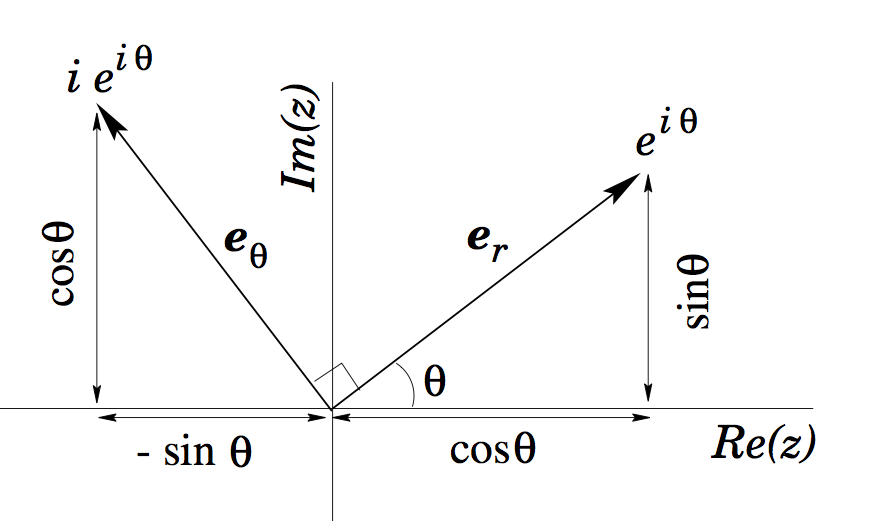
\includegraphics [scale=0.4] {Fitzpatrick1.png} \end{center}
it's clear that they are orthogonal.  If you do the dot product
\[ \mathbf{e}_{\theta} \cdot  \mathbf{e}_r = (\cos \theta + i \sin \theta) \cdot ( i\cos \theta - \sin \theta) \]
and, as long as you think of the $i$ as part of the unit vector, it works.

So now we have some position vector
\[ z = r e^{i \theta} \]
we differentiate and obtain
\[ \dot{z} = \dot{r} e^{i\theta} + r \dot{\theta} i e^{i \theta} \]
\[ = \dot{r} \mathbf{e}_r +  r \dot{\theta} \mathbf{e}_{\theta} \]
what this means is that the velocity has two components, the radial velocity
\[ \mathbf{v}_r = \dot{r} \mathbf{e}_r  \]
and the tangential velocity
\[ \mathbf{v}_{\theta} =  r \dot{\theta} = r \omega \]
Just so you are not thinking this is no big deal (see UCM) the great thing here is that we have not assumed that the velocity is perpendicular to the position vector.  It is a general result.  And in the case where $\dot{r} = 0$, we get the standard results.

Furthermore, we can do the acceleration in an analogous way.
\[ \dot{z} = \dot{r} e^{i\theta} + r \dot{\theta} i e^{i \theta} \]
\[ \ddot{z} = \dot{r}(\frac{d}{dt} e^{i\theta} ) +  \ddot{r}  e^{i\theta} + \dot{r} \dot{\theta} i e^{i \theta} +  r \ddot{\theta} i e^{i \theta} +  r \dot{\theta} i (\frac{d}{dt} e^{i\theta} )    \]
\[ = \dot{r} \dot{\theta} i e^{i \theta}  +  \ddot{r}  e^{i\theta} + \dot{r} \dot{\theta} i e^{i \theta} +  r \ddot{\theta} i e^{i \theta} +  r \dot{\theta} i  \dot{\theta} i e^{i \theta}    \]
\[ = (\ddot{r} - \dot{r} \dot{\theta}^2) e^{i\theta} + (2 \dot{r} \dot{\theta}  + \dot{r} \ddot{\theta}) i e^{i \theta}  \]
In other words, the acceleration has two components, the radial component
\[ \mathbf{a}_r = (\ddot{r} - \dot{r} \dot{\theta}^2) e^{i\theta} = (\ddot{r} - \dot{r} \dot{\theta}^2) \mathbf{e}_r = \ddot{r} - r \omega^2 \]
and the tangential component
\[ \mathbf{a}_{\theta} =  \dot{r} \ddot{\theta} + 2 \dot{r} \dot{\theta} = r \dot{\omega} + 2 \dot{r} \omega  \]
For UCM, then $\dot{r} = 0$ and
\[ \mathbf{a}_r = - r \omega^2 \]
\[ \mathbf{a}_{\theta} =  r \dot{\omega}  \]


\end{document}  